\documentclass[
    12pt,
    onehalfspacing,
    secnum,
]
{thepaper}


\usepackage{amsmath}
\usepackage{lipsum}
\usepackage{mhchem} % For chemical notation
\usepackage{siunitx}    % For SI units
\usepackage{gensymb}    % Symbols
\usepackage[misc]{ifsym} % For the \Letter symbol
\usepackage{tabularx}   % For making Knitr tables compatible
\usepackage{multirow}
\usepackage{multicol}

\bibliographystyle{aps}


%%%%%%%%%%%%%%%%%%%%%%%%%%%%%%%%%%%%%
%%%         TITLE PAGE
%%%%%%%%%%%%%%%%%%%%%%%%%%%%%%%%%%%%%
\title{My Awesome Template for Research Article}

\author[1]{Minjoon Hong}
\author[2, *]{Co-author}

% Affiliations
\affil[1]{School of Life Sciences, University of Sussex}
\affil[2]{University of Somewhere}

\begin{document}
\maketitle

\begin{abstract}
\lipsum[1]
\end{abstract}

%%%%%%%%%%%%%%%%%%%%%%%%%%%%%%%%%%%%%
%%%         MAIN TEXT
%%%%%%%%%%%%%%%%%%%%%%%%%%%%%%%%%%%%%
% \begin{multicols}{2}
\section{Introduction}
\lipsum[2-3]
This is citation.\cite{neese2018}

\subsection{Subsection 1}

\subsubsection{Subsubsection 1}

\paragraph{Paragraph 1}
\lipsum[4]

\begin{figure}[!htbp]
    \centering
    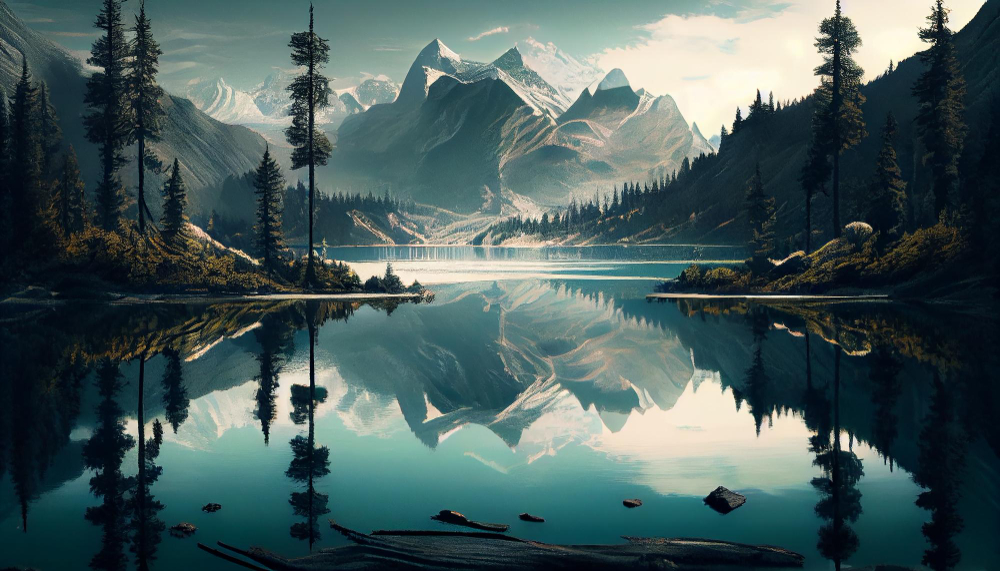
\includegraphics[width=0.6\textwidth]{src/images/example.jpg}
    \caption{This is a caption.}
\end{figure}


\begin{table}[h!]
    \centering
    \begin{tabular}{c c c c} 
     \hline
     Col1 & Col2 & Col2 & Col3 \\ 
     \hline
     1 & 6 & 87837 & 787 \\ 
     2 & 7 & 78 & 5415 \\
     3 & 545 & 778 & 7507 \\
     4 & 545 & 18744 & 7560 \\
     5 & 88 & 788 & 6344 \\
     \hline
    \end{tabular}
    \caption{Table to test captions and labels.}
    \label{table:1}
\end{table}
\bibliography{main}
% \end{multicols}

\end{document}
